\documentclass[handout,aspectratio=169]{beamer}
\useoutertheme{split}
\useinnertheme{circles}
\usecolortheme{custom}
\setbeamertemplate{navigation symbols}{}
\graphicspath{{graphics/}}

\usepackage{mathtools}

\newcommand*\oldmacro{}%
\let\oldmacro\insertshorttitle%
\renewcommand*\insertshorttitle{%
	\oldmacro\hspace{3.6cm}%
	    \insertframenumber\,/\,\inserttotalframenumber}

\title{Cache for HLS}
\subtitle{A multi-process architecture}
\author{Brignone Giovanni}
\titlegraphic{
\includegraphics[width=.2\textwidth]{polito_logo.png}}
%\institute{Politecnico di Torino}
\date{June 7, 2021}

\AtBeginSection[] {
	\tableofcontents[
		currentsection,
		sectionstyle=show/shaded,
		subsectionstyle=show/show/hide
	]
}

\begin{document}
\begin{frame}
	\maketitle
\end{frame}

\section{Introduction}
\subsection{Motivation}
\begin{frame}{Motivation}
	\begin{itemize}[<+->]
		\item \textbf{Problem}:\\
			big arrays mapped to \highlight{DRAM} $\Rightarrow$
			performance \highlight{bottlenecks}
		\item \textbf{Proposed solution}:\\
			cache module designed to:
			\begin{itemize}[<.->]
				\item exploit \highlight{BRAMs}
				\item \highlight{easily integrable} into any
					\emph{Vitis HLS} design
				\item have an \highlight{high hit ratio}
			\end{itemize}
	\end{itemize}
\end{frame}

\section{Architecture}
\subsection{Inlined architecture}
\begin{frame}{Inlined architecture (Ma Liang)}
	\begin{minipage}{.7\textwidth}
		\begin{center}
			Array access $\rightarrow$ Inlined cache logic
		\end{center}

		\bigskip

		\begin{itemize}
			\item cache logic mixed with application logic
			\item one cache per array
			\item single-port only
		\end{itemize}
	\end{minipage}
	\begin{minipage}{.28\textwidth}
		\begin{center}
			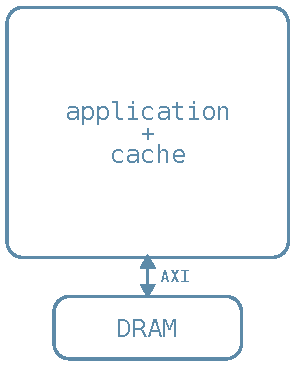
\includegraphics[width=.8\textwidth]{liang_arch.pdf}
		\end{center}
	\end{minipage}
\end{frame}
\subsection{Multi-process architecture}
\begin{frame}{Multi-process architecture}
	\begin{minipage}{.7\textwidth}
		\begin{center}
			Array access $\rightarrow$ Request to separate module
		\end{center}
		\begin{itemize}
			\item decoupling between application and cache logic
				(communication through FIFOs)
			\item one cache per array
			\item may support multiple ports (work in progress)
		\end{itemize}
	\end{minipage}
	\begin{minipage}{.28\textwidth}
		\begin{center}
			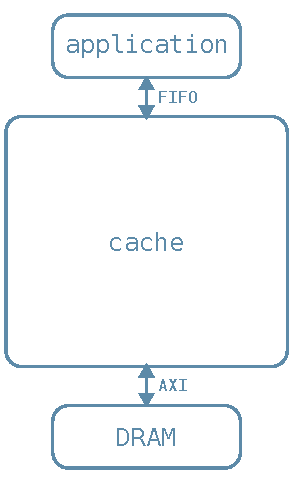
\includegraphics[width=.8\textwidth]{complete_arch.pdf}
		\end{center}
	\end{minipage}
\end{frame}

\section{Implementation}
\subsection{Tools}
\begin{frame}{Tools}
	\texttt{C++} code coupled with \emph{Vitis HLS} (2020.2) allow:
	\pause
	\begin{itemize}[<+->]
		\item \textbf{Multiple processes modeling}:\\
			infinite loops parallelized by:
			\begin{itemize}
				\item<.-> \underline{SW simulation:} \texttt{std::thread}
				\item<.-> \underline{Synthesis:} \texttt{DATAFLOW} with
					\textit{start propagation} disabled
			\end{itemize}
		\item \textbf{Inter-process communication}: \texttt{hls::stream} FIFOs
		\item \textbf{Performance optimization}:
			\begin{itemize}
				\item<.-> loop pipelining: new request each cycle
				\item<.-> automatic port widening: access one line at a time in DRAM
			\end{itemize}
		\item \textbf{Customization:} cache parameters set through \texttt{template}
		\item \textbf{Limitations}: cannot override ``\texttt{[]~operator}''
			for \texttt{set} due to automatic \texttt{class} disaggregation
	\end{itemize}
\end{frame}

\subsection{Internal architecture}
\begin{frame}{Internal architecture}
	\begin{minipage}{.7\textwidth}
		\begin{itemize}[<+->]
			\item \textbf{Problem}: persuade HLS to \highlight{schedule
				cache HIT response early} in the pipeline
			\item \textbf{Proposed solution}: split the cache into
				\highlight{two processes}:
			\begin{enumerate}[<.->]
				\item \texttt{core}:
					\begin{itemize}
						\item manage requests from \texttt{application}
						\item keep cache data structures up-to-date
					\end{itemize}
				\item \texttt{mem\_if}:
					\begin{itemize}
						\item manage requests from \texttt{core}
						\item access DRAM
					\end{itemize}
			\end{enumerate}
			\pause[\thebeamerpauses]
				\begin{center}
					$\Rightarrow$ \highlight{synthesizer job} is \highlight{simplified}:\\
					HIT response scheduled earlier
				\end{center}
	\end{itemize}
	\end{minipage}
	\onslide<1->
	\begin{minipage}{.28\textwidth}
		\begin{center}
			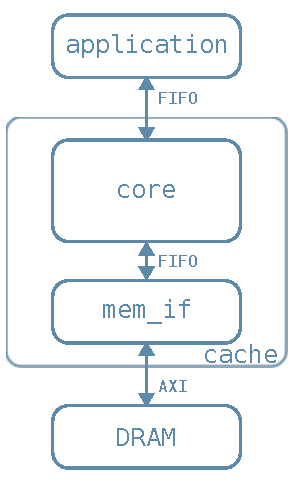
\includegraphics[width=.8\textwidth]{internal_arch.pdf}
		\end{center}
	\end{minipage}
\end{frame}
\begin{frame}{\texttt{mem\_if} implementation}
	\framesubtitle{Functionality}
	\begin{minipage}{.7\textwidth}
		Manage DRAM accesses:
		\begin{enumerate}
			\item read request from \texttt{core}
			\item access DRAM
			\item write response to \texttt{core}
				(if \texttt{read} request)
		\end{enumerate}
	\end{minipage}
	\begin{minipage}{.28\textwidth}
		\begin{center}
			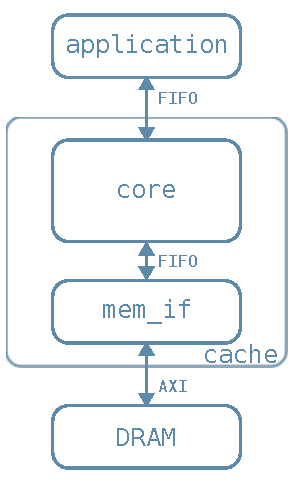
\includegraphics[width=.8\textwidth]{internal_arch.pdf}
		\end{center}
	\end{minipage}
\end{frame}
\begin{frame}{\texttt{core} implementation}
	\framesubtitle{Functionality}
	\begin{minipage}{.7\textwidth}
		\begin{enumerate}[<+->]
			\item read request from \texttt{application}
			\item<.-> check if it is an HIT or a MISS
			\item if MISS: 
				\begin{itemize}
					\item issue a \texttt{write} request of
						the line to be replaced to
						\texttt{mem\_if} (if write-back
						is necessary)
					\item issue a \texttt{read} request of the
						line to be loaded to \texttt{mem\_if}
					\item<.-> read \texttt{mem\_if} response and
						update BRAM

				\end{itemize}
			\item access BRAM
			\item<.-> write response to \texttt{application}
				(if \texttt{read})
		\end{enumerate}
	\end{minipage}
	\begin{minipage}{.28\textwidth}
		\begin{center}
			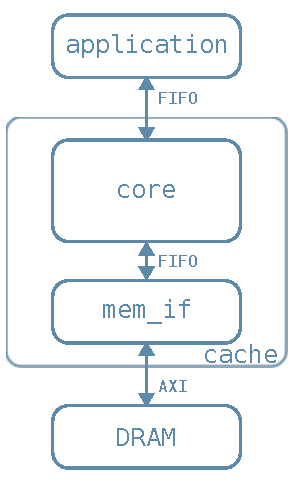
\includegraphics[width=.8\textwidth]{internal_arch.pdf}
		\end{center}
	\end{minipage}
\end{frame}
\subsection{Problems and solutions}
\begin{frame}{BRAM dependencies~-~Line loading}
	\framesubtitle{}
	\begin{minipage}{.7\textwidth}
		\begin{itemize}[<+->]
			\item \textbf{Problem}:
				\highlight{reading BRAM} line immediately
				\highlight{after it has been loaded} from DRAM
				causes a \emph{Read-After-Write} dependency
			\item \textbf{Proposed solution}:
				store the \texttt{mem\_if} response in a
				\highlight{buffer} which can be immediately
				accessed and update BRAM afterwards
		\end{itemize}
	\end{minipage}
	\onslide<1->
	\begin{minipage}{.28\textwidth}
		\begin{center}
			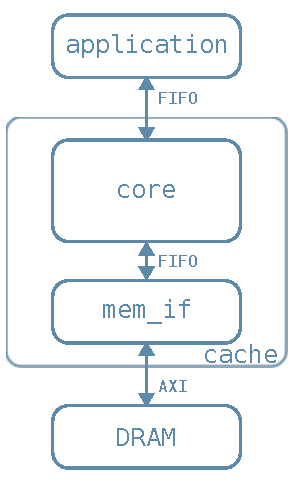
\includegraphics[width=.8\textwidth]{internal_arch.pdf}
		\end{center}
	\end{minipage}
\end{frame}
\begin{frame}{BRAM dependencies~-~RAW \texttt{request}}
	\begin{minipage}{.7\textwidth}
		\begin{itemize}[<+->]
			\item \textbf{Problem}:
				a \highlight{\texttt{write request}} immediately
				followed by a \highlight{\texttt{read request}}
				to the same element causes a \emph{Read-After-Write}
				dependency on BRAM
			\item \textbf{Proposed solution}:
				\texttt{raw\_cache} inside \texttt{cache}:
				\begin{itemize}[<.->]
					\item \texttt{write} request: store the
						written line to a buffer
					\item subsequent \texttt{read} request to
						the same line: \highlight{access
						the buffer instead of BRAM}
				\end{itemize}
		\end{itemize}
	\end{minipage}
	\onslide<1->
	\begin{minipage}{.28\textwidth}
		\begin{center}
			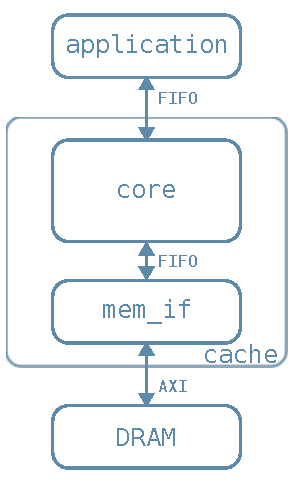
\includegraphics[width=.8\textwidth]{internal_arch.pdf}
		\end{center}
	\end{minipage}
\end{frame}
\begin{frame}{Request optimization}
	\begin{minipage}{.7\textwidth}
		\begin{itemize}[<+->]
			\item \textbf{Problem}:
				\begin{itemize}[<.->]
					\item each \highlight{FIFO access} costs
						\highlight{1 cycle}
					\item accesses to arrays are often sequential
				\end{itemize}
			\item \textbf{Proposed solution}:
				\texttt{l1\_cache} in the interface (\texttt{application}
				side):
				\begin{itemize}[<.->]
					\item \texttt{read} request:
						\highlight{get the whole cache line},
						store it in a buffer and return
						the requested element
					\item subsequent \texttt{read} request to the same
						line: access the \highlight{buffer}
				\end{itemize}
				$\Rightarrow$ \highlight{avoid passing through FIFOs}
		\end{itemize}
	\end{minipage}
	\onslide<1->
	\begin{minipage}{.28\textwidth}
		\begin{center}
			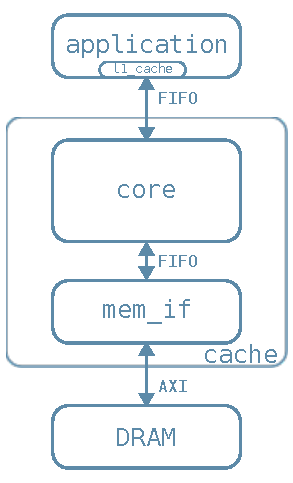
\includegraphics[width=.8\textwidth]{l1_arch.pdf}
		\end{center}
	\end{minipage}
\end{frame}
\section{Results}
\subsection{Performance}
\begin{frame}{Performance}
	\begin{itemize}
		\item \textbf{Loop pipelining}:
			\begin{itemize}
				\item \texttt{core}: $II=1$
				\item \texttt{mem\_if}: $II=\left\lceil \frac{line\_size}{AXI\_if\_size} \right\rceil$
			\end{itemize}
		\item \textbf{L1 HIT}: latency of 1 cycle
		\item \textbf{HIT}: latency of 6 cycles
	\end{itemize}
\end{frame}
\subsection{Matrix Multiplication}
\begin{frame}{Matrix Multiplication}
	\begin{minipage}{.77\textwidth}
		\begin{itemize}
			\item $A$ matrix: each row accessed $n$ times:
				$hit\_ratio = \frac{(line\_size \cdot x) - 1}{line\_size \cdot x},
				x = \begin{cases}
					1, & line\_size < m \\
					n, & otherwise
				\end{cases}$
			\item<.-> $C$ matrix
				accessed by rows:
				$hit\_ratio = \frac{line\_size - 1}{line\_size}$
		\end{itemize}
	\end{minipage}
	\begin{minipage}{.22\textwidth}
		\begin{center}
			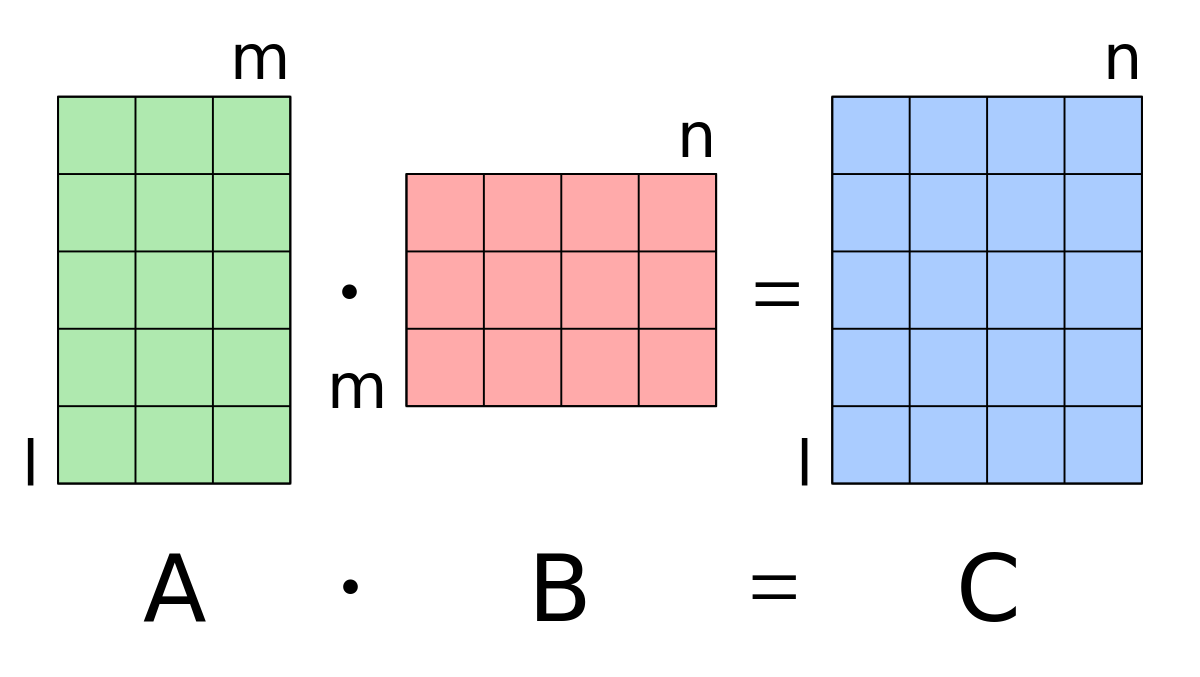
\includegraphics[width=.9\textwidth]{matmul.png}
		\end{center}
	\end{minipage}
\end{frame}
\begin{frame}{Matrix Multiplication}
	\begin{minipage}{.77\textwidth}
		\begin{itemize}
			\item $B$ matrix accessed by columns:\\
				modified \emph{direct mapped}
				address mapping:

				\begin{center}
					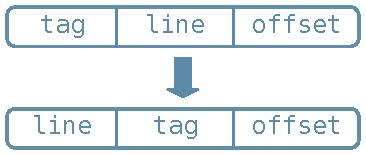
\includegraphics[width=.3\textwidth]{mmul_addr.pdf}
				\end{center}

				\bigskip
				$\Rightarrow \begin{cases}
					hit\_ratio = \frac{(line\_size \cdot x) - 1}{line\_size \cdot x} \\
				x = \begin{cases}
					0, & n\_lines < m \\
					1, & n\_lines \geq m \wedge line\_size < n \\
					l, & n\_lines \geq m \wedge line\_size \geq n \\
				\end{cases}
				\end{cases}$
		\end{itemize}
	\end{minipage}
	\begin{minipage}{.22\textwidth}
		\begin{center}
			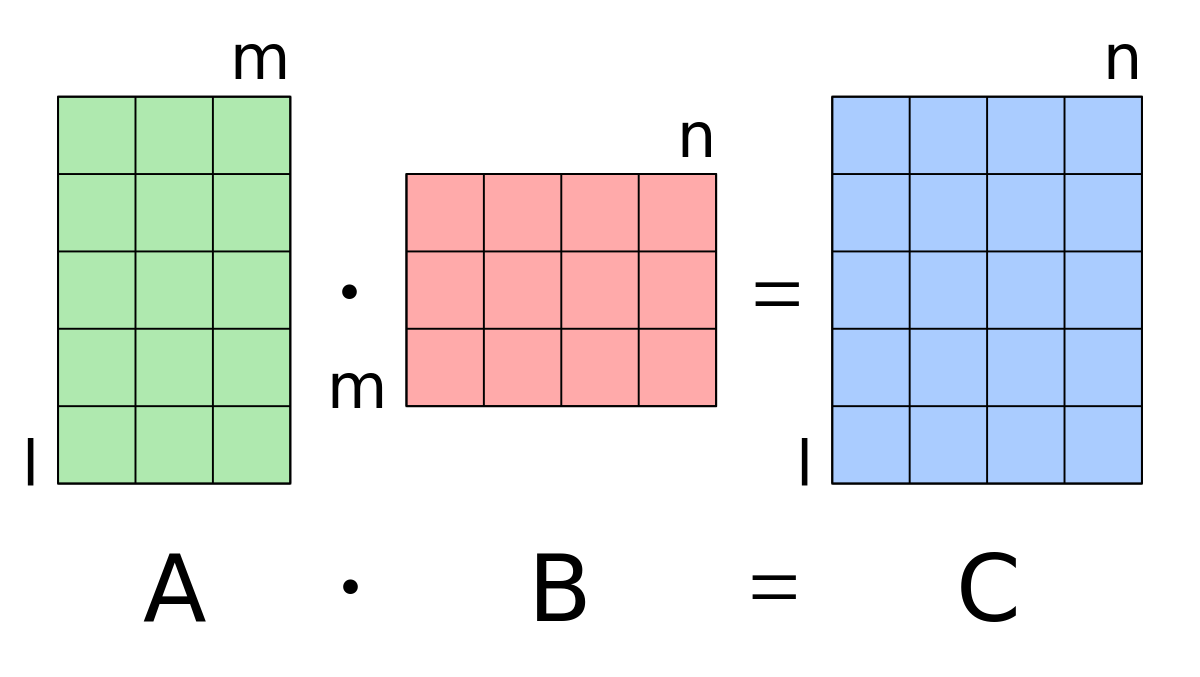
\includegraphics[width=.9\textwidth]{matmul.png}
		\end{center}
	\end{minipage}
\end{frame}
\begin{frame}{Matrix Multiplication}
	\framesubtitle{Practical example}
	\begin{minipage}{.77\textwidth}
		\begin{itemize}
			\item \textbf{Problem size}:\\
				$\begin{cases}
					l &= 16 \\
					m &= 32 \\
					n &= 64 \\
				\end{cases}$
			\item \textbf{Caches size}:\\
				$\begin{rcases}
					n\_lines_A = 2, & line\_size_A = 32 \\
					n\_lines_B = m, & line\_size_B = 32 \\
					n\_lines_C = 2, & line\_size_C = 32 \\
				\end{rcases}
				\Rightarrow
				\begin{cases}
					hit\_ratio_A \simeq 100\% \\
					hit\_ratio_B = 96.9\% \\
					hit\_ratio_C = 96.9\% \\
				\end{cases}$
		\end{itemize}
	\end{minipage}
	\onslide<1->
	\begin{minipage}{.22\textwidth}
		\begin{center}
			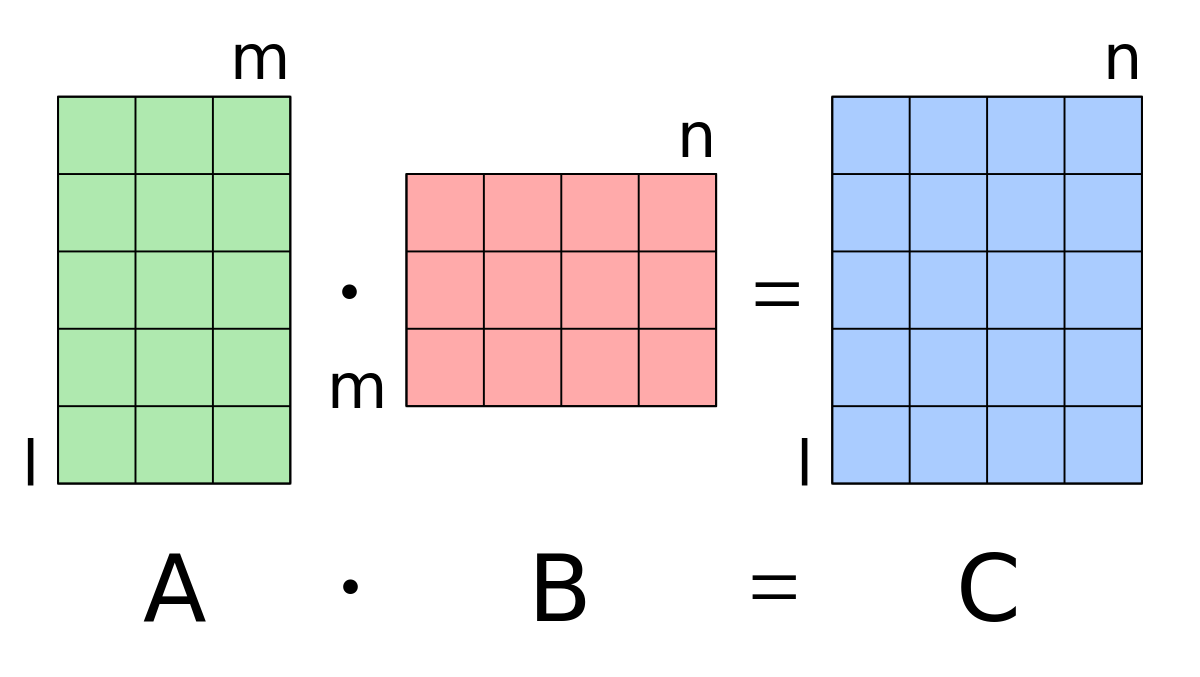
\includegraphics[width=.9\textwidth]{matmul.png}
		\end{center}
	\end{minipage}
\end{frame}
\begin{frame}{Matrix Multiplication}
	\framesubtitle{Practical example}
	\begin{minipage}{.77\textwidth}
		\begin{itemize}
			\item \textbf{Execution time without caches}:\\ $2,428,745 \mu s$
			\item \textbf{Execution time with caches}:\\ $1,160,105 \mu s$
		\end{itemize}
		\begin{center}
			$\Rightarrow$ execution is $2.1x$ faster
		\end{center}
	\end{minipage}
	\onslide<1->
	\begin{minipage}{.22\textwidth}
		\begin{center}
			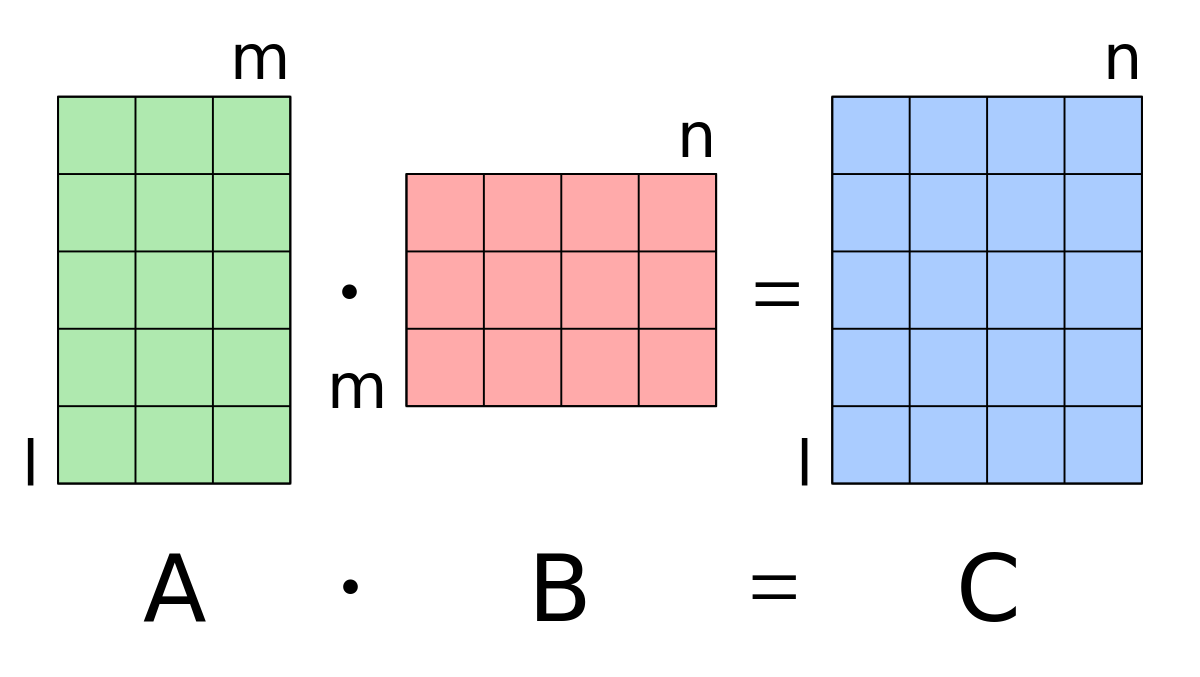
\includegraphics[width=.9\textwidth]{matmul.png}
		\end{center}
	\end{minipage}
\end{frame}
\begin{frame}{Matrix Multiplication}
	\framesubtitle{Reference example}
	\begin{minipage}{.77\textwidth}
		\begin{itemize}
			\item \textbf{Problem size}:\\
				$\begin{cases}
					l &= 16 \\
					m &= 32 \\
					n &= 64 \\
				\end{cases}$
			\item \textbf{Caches size}:\\
				$\begin{rcases}
					n\_lines_A = l, & line\_size_A = m \\
					n\_lines_B = m, & line\_size_B = n \\
					n\_lines_C = l, & line\_size_C = n \\
				\end{rcases}
				\Rightarrow
				\begin{cases}
					hit\_ratio_A \simeq 100\% \\
					hit\_ratio_B = 99.9\% \\
					hit\_ratio_C = 98.4\% \\
				\end{cases}$
		\end{itemize}
	\end{minipage}
	\onslide<1->
	\begin{minipage}{.22\textwidth}
		\begin{center}
			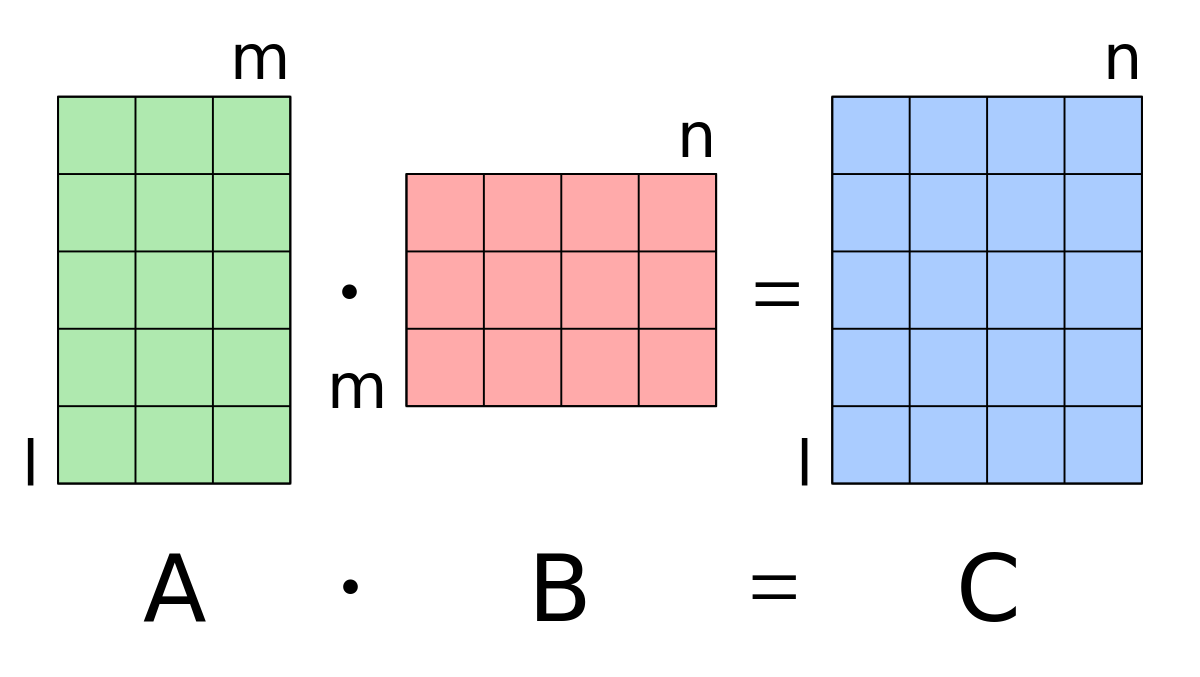
\includegraphics[width=.9\textwidth]{matmul.png}
		\end{center}
	\end{minipage}
\end{frame}
\begin{frame}{Matrix Multiplication}
	\framesubtitle{Reference example}
	\begin{minipage}{.77\textwidth}
		\begin{itemize}
			\item \textbf{Execution time without caches}:\\ $2,428,745 \mu s$
			\item \textbf{Execution time with caches}:\\ $369,045 \mu s$
		\end{itemize}
		\begin{center}
			$\Rightarrow$ execution is $6.6x$ faster
		\end{center}
	\end{minipage}
	\onslide<1->
	\begin{minipage}{.22\textwidth}
		\begin{center}
			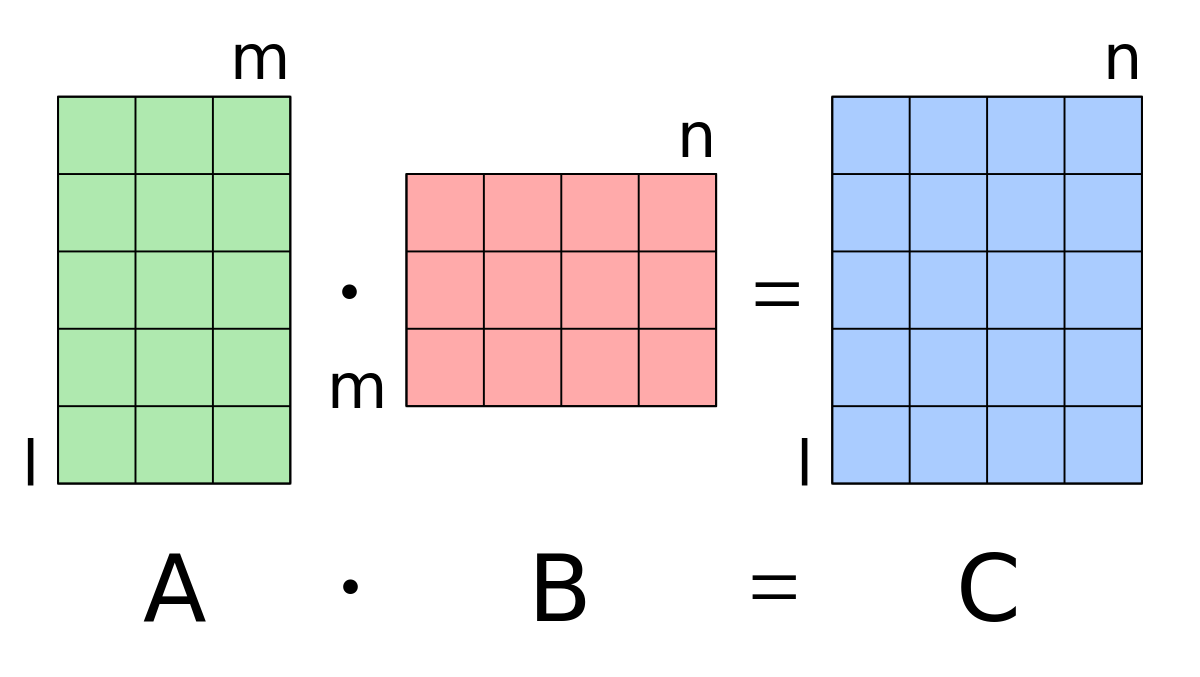
\includegraphics[width=.9\textwidth]{matmul.png}
		\end{center}
	\end{minipage}
\end{frame}

\section{Future work}
\subsection{Multi-port cache}
\begin{frame}{Multi-port cache}
	\begin{itemize}[<+->]
		\item \textbf{Problem}: cache manages one request per cycle
			$\Rightarrow$ \highlight{unrolling} a loop which uses the cache is not
			trivial
		\item \textbf{Possible workarounds}:
			access \highlight{multiple data elements for each request}
			and do all the unroll in \texttt{application}; two possible ways:
			\begin{itemize}[<.->]
				\item \texttt{get\_line}: return a whole cache
					line
				\item pack multiple data elements in a single
					cache element (e.g. \texttt{hls::vector})
			\end{itemize}
		\item \textbf{Proposed solution}: provide \highlight{$N$ ports},
			where $N$ is the unroll factor
	\end{itemize}
\end{frame}
\begin{frame}{Multi-port cache}
	\framesubtitle{Implementation}
	\begin{minipage}{.7\textwidth}
		\begin{itemize}[<+->]
			\item \textbf{Straightforward implementation}:
				\begin{itemize}[<.->]
					\item provide $N$ FIFOs on the interface
					\item \highlight{unroll \texttt{core}}
						loop by a factor $N$
				\end{itemize}
			\item \textbf{Problem}: all the $N$ requests may
				\highlight{refer to the same line}
				$\rightarrow$ each iteration must wait completion of
				previous one
		\end{itemize}
	\end{minipage}
	\onslide<1->
	\begin{minipage}{.28\textwidth}
		\begin{center}
			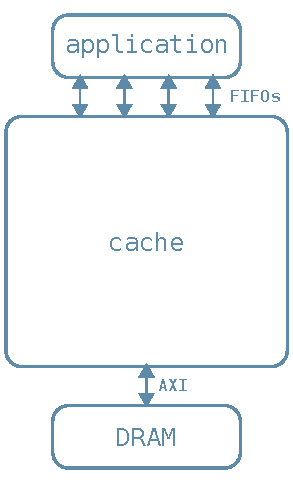
\includegraphics[width=.8\textwidth]{multiport_arch.pdf}
		\end{center}
	\end{minipage}
\end{frame}
\begin{frame}{Multi-port cache}
	\framesubtitle{Implementation}
	\begin{minipage}{.7\textwidth}
		\begin{itemize}[<+->]
			\item \textbf{Proposed solution}:
				\begin{enumerate}[<.->]
					\item read all the $N$ requests
					\item check if they are all HIT
					\item if at least one MISS issue all the requests
						to \texttt{mem\_if}
					\item access BRAM
					\item write all the responses
				\end{enumerate}
				\pause[\thebeamerpauses]
				\begin{itemize}
					\item cache addressing mode converted to an
						associative one
					\item possibly implement \texttt{core}
						at RTL to have full control
						on scheduling
				\end{itemize}
		\end{itemize}
	\end{minipage}
	\onslide<1->
	\begin{minipage}{.28\textwidth}
		\begin{center}
			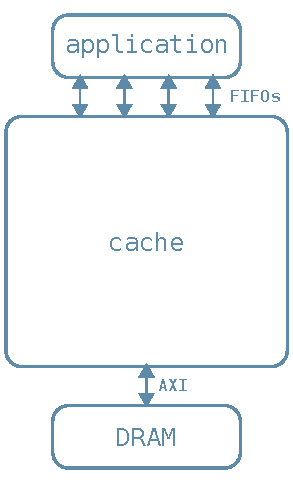
\includegraphics[width=.8\textwidth]{multiport_arch.pdf}
		\end{center}
	\end{minipage}
\end{frame}

\section*{Summary}
\begin{frame}{Summary}
	\begin{minipage}{.7\textwidth}
		\begin{itemize}
			\item \textbf{Architecture}: \emph{Divide et Impera}
			\item \textbf{Results}:
				good single-port pipeline performance
			\item \textbf{Future work}: ease \texttt{application} unroll
		\end{itemize}
	\end{minipage}
	\begin{minipage}{.28\textwidth}
		\begin{center}
			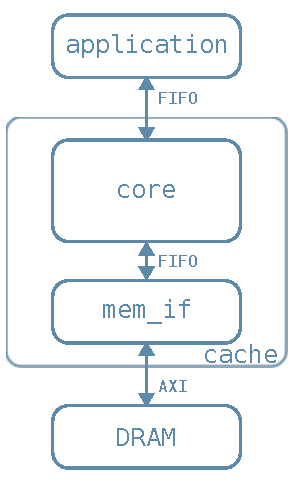
\includegraphics[width=.8\textwidth]{internal_arch.pdf}
		\end{center}
	\end{minipage}
\end{frame}

\end{document}

